% ==============================================================================
% HEMS Optimization using Data Science - Beamer Presentation
% Author: Samuel Heinrich
% Course: ITS8080 Energy Data Science
% ==============================================================================

\documentclass[aspectratio=169,11pt]{beamer}

% Theme and styling
\usetheme{Madrid}
\usecolortheme{default}

% Color definitions
\definecolor{energyblue}{RGB}{31,119,180}
\definecolor{pvgreen}{RGB}{44,160,44}
\definecolor{priceorange}{RGB}{255,165,0}
\definecolor{storygray}{RGB}{127,127,127}

% Fix: Make frame titles visible with proper foreground colors
\setbeamercolor{title}{fg=white,bg=energyblue}
\setbeamercolor{frametitle}{fg=white,bg=energyblue}
\setbeamercolor{structure}{fg=energyblue}
\setbeamercolor{block title}{bg=energyblue!80,fg=white}
\setbeamercolor{block body}{bg=energyblue!10}
\setbeamercolor{section in toc}{fg=energyblue}
\setbeamercolor{subsection in toc}{fg=energyblue!80}
\setbeamercolor{item}{fg=energyblue}

% Packages
\usepackage[utf8]{inputenc}
\usepackage[T1]{fontenc}
\usepackage{amsmath,amssymb,amsfonts}
\usepackage{graphicx}
\usepackage{booktabs}
\usepackage{tikz}
\usetikzlibrary{shapes,arrows,positioning,calc}
\usepackage{hyperref}
\usepackage{xcolor}
\usepackage{multicol}

% Graphics path
\graphicspath{{figures/}}

% Title information
\title[HEMS Optimization]{\textbf{HEMS Optimization using Data Science}}
\subtitle{Home Energy Management System with Battery Storage}
\author{Samuel Heinrich}
\institute[ITS8080]{Course: ITS8080 Energy Data Science}
\date{\today}

\begin{document}

% ==============================================================================
% TITLE SLIDE
% ==============================================================================
\begin{frame}
    \titlepage
\end{frame}

% ==============================================================================
% OUTLINE
% ==============================================================================
\begin{frame}{Agenda}
    \tableofcontents
\end{frame}

% ==============================================================================
% SECTION 1: INTRODUCTION
% ==============================================================================
\section{Introduction \& Problem Statement}

\begin{frame}{The Energy Trilemma}
    \begin{columns}[T]
        \begin{column}{0.55\textwidth}
            \textbf{Three competing objectives:}
            \begin{enumerate}
                \item \textcolor{energyblue}{\textbf{Security}} -- Reliable energy supply
                \item \textcolor{pvgreen}{\textbf{Sustainability}} -- Low carbon emissions
                \item \textcolor{priceorange}{\textbf{Equity}} -- Affordable energy access
            \end{enumerate}

            \vspace{1em}
            \textbf{Challenge:} Balancing all three requires intelligent coordination of distributed energy resources (DERs).

            \vspace{1em}
            \textbf{Context:} Digitalization of energy systems enables smart grid integration and demand-side management.
        \end{column}
        \begin{column}{0.45\textwidth}
            \begin{center}
                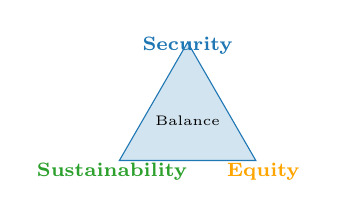
\begin{tikzpicture}[scale=0.8]
                    \node[draw=energyblue, fill=energyblue!20, minimum size=2cm, regular polygon, regular polygon sides=3] at (0,0) {};
                    \node[font=\scriptsize\bfseries, text=energyblue] at (0,1.2) {Security};
                    \node[font=\scriptsize\bfseries, text=pvgreen] at (-1.2,-0.8) {Sustainability};
                    \node[font=\scriptsize\bfseries, text=priceorange] at (1.2,-0.8) {Equity};
                    \node[font=\tiny] at (0,0) {Balance};
                \end{tikzpicture}
            \end{center}
        \end{column}
    \end{columns}
\end{frame}

\begin{frame}{The ``Duck Curve'' Problem}
    \begin{columns}[T]
        \begin{column}{0.45\textwidth}
            \textbf{PV/Demand Mismatch:}
            \begin{itemize}
                \item PV generation peaks at solar noon
                \item Household demand peaks in evening hours
                \item \textbf{Peak Coincidence:} High price correlates with high demand
            \end{itemize}

            \vspace{0.5em}
            \textbf{Consequences:}
            \begin{itemize}
                \item Grid stress during evening ramp-up
                \item PV curtailment during midday surplus
                \item Higher electricity costs for consumers
            \end{itemize}
        \end{column}
        \begin{column}{0.55\textwidth}
            \begin{center}
                \includegraphics[width=\textwidth]{03_timeseries_overlay.png}
            \end{center}
        \end{column}
    \end{columns}
\end{frame}

\begin{frame}{Project Goal: Home Energy Management System (HEMS)}
    \begin{block}{Objective}
        Develop an intelligent HEMS that uses \textbf{forecasting} and \textbf{optimization} to minimize energy costs while maximizing PV self-consumption.
    \end{block}

    \vspace{0.5em}
    \begin{columns}[T]
        \begin{column}{0.5\textwidth}
            \textbf{System Components:}
            \begin{itemize}
                \item PV System: 5 kW capacity
                \item Battery Storage: 10 kWh capacity
                \item Grid Connection: 5 kW max flow
                \item Smart Controller (this project)
            \end{itemize}
        \end{column}
        \begin{column}{0.5\textwidth}
            \textbf{Data-Driven Approach:}
            \begin{enumerate}
                \item Forecast demand using ML models
                \item Optimize battery dispatch via LP
                \item Maximize self-consumption
                \item Minimize grid import costs
            \end{enumerate}
        \end{column}
    \end{columns}
\end{frame}

% ==============================================================================
% SECTION 2: DATA ANALYSIS
% ==============================================================================
\section{Data Analysis}

\begin{frame}{Dataset Overview}
    \begin{columns}[T]
        \begin{column}{0.4\textwidth}
            \textbf{Hourly Time Series Data:}
            \begin{itemize}
                \item \textcolor{energyblue}{\textbf{Demand}} (kWh)
                \item \textcolor{pvgreen}{\textbf{PV Generation}} (kWh)
                \item \textcolor{priceorange}{\textbf{Price}} (€/kWh)
                \item \textbf{Weather:} Temp, Irradiance
            \end{itemize}

            \vspace{0.5em}
            \textbf{Key Observations:}
            \begin{itemize}
                \item Demand: Right-skewed
                \item PV: Zero-inflated
                \item Clear 24h diurnal patterns
            \end{itemize}
        \end{column}
        \begin{column}{0.6\textwidth}
            \begin{center}
                \includegraphics[width=\textwidth]{03_distributions.png}
            \end{center}
        \end{column}
    \end{columns}
\end{frame}

\begin{frame}{Exploratory Data Analysis: Temporal Patterns}
    \begin{columns}[T]
        \begin{column}{0.5\textwidth}
            \begin{center}
                \includegraphics[width=\textwidth]{03_typical_profiles.png}
            \end{center}
        \end{column}
        \begin{column}{0.5\textwidth}
            \begin{center}
                \includegraphics[width=\textwidth]{06_monthly_hourly_heatmap.png}
            \end{center}
        \end{column}
    \end{columns}

    \vspace{0.3em}
    \begin{center}
        \textbf{Key Insight:} Strong 24h seasonality with distinct weekday/weekend patterns
    \end{center}
\end{frame}

\begin{frame}{Data Cleaning: PV Sensor Imputation}
    \begin{columns}[T]
        \begin{column}{0.42\textwidth}
            \textbf{Problem:} PV sensors had missing data.

            \vspace{0.5em}
            \textbf{Methods Compared:}
            \begin{enumerate}
                \item \textbf{Linear Interpolation}
                \item \textbf{STL Decomposition}
                \item \textbf{KNN Multivariate}
            \end{enumerate}

            \vspace{0.5em}
            \textbf{Selection Criteria:}
            \begin{itemize}
                \item Variance preservation
                \item Peak value accuracy
                \item Physical plausibility
            \end{itemize}

            \vspace{0.5em}
            \textcolor{pvgreen}{\textbf{Winner: KNN Multivariate}}
        \end{column}
        \begin{column}{0.58\textwidth}
            \begin{center}
                \includegraphics[width=\textwidth]{04_imputation_overlay.png}
            \end{center}
        \end{column}
    \end{columns}
\end{frame}

\begin{frame}{Feature Engineering}
    \begin{columns}[T]
        \begin{column}{0.5\textwidth}
            \textbf{Time Features (Cyclic Encoding):}
            \begin{align*}
                \text{hour\_sin} &= \sin\left(\frac{2\pi \cdot \text{hour}}{24}\right) \\
                \text{hour\_cos} &= \cos\left(\frac{2\pi \cdot \text{hour}}{24}\right)
            \end{align*}

            \textbf{Calendar Features:}
            \begin{itemize}
                \item Weekend boolean indicator
                \item Day of week
            \end{itemize}

            \textbf{Weather-Derived Features:}
            \begin{itemize}
                \item Heating Degree Days (HDD)
                \item Cooling Degree Days (CDD)
            \end{itemize}
        \end{column}
        \begin{column}{0.5\textwidth}
            \textbf{Feature Importance (Correlation with Demand):}
            \vspace{0.5em}

            \begin{tabular}{lc}
                \toprule
                \textbf{Feature} & \textbf{Correlation} \\
                \midrule
                hour\_sin & 0.233 \\
                Price & 0.228 \\
                hour\_cos & 0.221 \\
                DNI (W/m²) & 0.097 \\
                Diffuse Radiation & 0.094 \\
                Heating Degree & 0.053 \\
                \bottomrule
            \end{tabular}

            \vspace{0.5em}
            \textcolor{energyblue}{\textbf{Key: Time-of-day is the \#1 predictor!}}
        \end{column}
    \end{columns}
\end{frame}

% ==============================================================================
% SECTION 3: MODELING
% ==============================================================================
\section{Modeling Approach}

\begin{frame}{Time Series Decomposition: STL}
    \begin{columns}[T]
        \begin{column}{0.35\textwidth}
            \textbf{STL Decomposition:}
            \[
                y_t = T_t + S_t + R_t
            \]

            \begin{itemize}
                \item $T_t$ -- Trend
                \item $S_t$ -- Seasonal (24h)
                \item $R_t$ -- Residual
            \end{itemize}

            \vspace{0.5em}
            \textbf{Key Finding:}\\
            \textcolor{energyblue}{24h seasonality dominant}

            \vspace{0.5em}
            Justifies SARIMA ($m=24$) and lag features for XGBoost.
        \end{column}
        \begin{column}{0.65\textwidth}
            \begin{center}
                \includegraphics[width=\textwidth]{06_stl_decomposition.png}
            \end{center}
        \end{column}
    \end{columns}
\end{frame}

\begin{frame}{Model Selection: Statistical vs. Machine Learning}
    \begin{columns}[T]
        \begin{column}{0.5\textwidth}
            \textbf{SARIMA Model:}
            \[
                \text{SARIMA}(1,1,1)(1,1,1)_{24}
            \]

            \begin{itemize}
                \item Classical statistical approach
                \item Captures seasonal patterns
                \item Interpretable coefficients
                \item \textcolor{priceorange}{nRMSE = 0.199}
            \end{itemize}
        \end{column}
        \begin{column}{0.5\textwidth}
            \textbf{XGBoost Model:}
            \begin{itemize}
                \item Gradient boosting ensemble
                \item Uses lag features + exogenous
                \item Handles non-linearities
                \item \textcolor{pvgreen}{\textbf{nRMSE = 0.166}}
            \end{itemize}

            \vspace{0.5em}
            \textbf{Key Features:}
            \begin{itemize}
                \item Lag 1, 2, 3, 24, 48 hours
                \item Cyclic time encoding
                \item Weather variables
            \end{itemize}
        \end{column}
    \end{columns}

    \vspace{1em}
    \begin{center}
        \colorbox{pvgreen!20}
        }
    \end{center}
\end{frame}

\begin{frame}{Evaluation Metric: Normalized RMSE}
    \begin{block}{Root Mean Square Error (RMSE)}
        \[
            \text{RMSE} = \sqrt{\frac{1}{n}\sum_{t=1}^{n}(y_t - \hat{y}_t)^2}
        \]
    \end{block}

    \begin{block}{Normalized RMSE (nRMSE)}
        \[
            \text{nRMSE} = \frac{\text{RMSE}}{\bar{y}} = \frac{\sqrt{\frac{1}{n}\sum_{t=1}^{n}(y_t - \hat{y}_t)^2}}{\frac{1}{n}\sum_{t=1}^{n}y_t}
        \]
    \end{block}

    \vspace{0.5em}
    \textbf{Interpretation:}
    \begin{itemize}
        \item nRMSE normalizes by the mean, enabling cross-series comparison
        \item Lower is better -- XGBoost: 0.166 vs SARIMA: 0.199
    \end{itemize}
\end{frame}

% ==============================================================================
% SECTION 4: FORECASTING RESULTS
% ==============================================================================
\section{Forecasting Results}

\begin{frame}{Walk-Forward Validation}
    \begin{columns}[T]
        \begin{column}{0.4\textwidth}
            \textbf{Methodology:}
            \begin{itemize}
                \item 7-day rolling horizon
                \item Expanding window retraining
                \item Avoids data leakage
            \end{itemize}

            \vspace{0.5em}
            \textbf{Baselines Compared:}
            \begin{enumerate}
                \item Naive (lag-1)
                \item Seasonal Naive (lag-24)
                \item SARIMA
                \item XGBoost
            \end{enumerate}
        \end{column}
        \begin{column}{0.6\textwidth}
            \begin{center}
                \includegraphics[width=\textwidth]{09_week_overlay_best.png}
            \end{center}
        \end{column}
    \end{columns}
\end{frame}

\begin{frame}{Model Comparison Results}
    \begin{columns}[T]
        \begin{column}{0.45\textwidth}
            \textbf{Performance Metrics:}
            \vspace{0.3em}

            \begin{table}
                \centering\footnotesize
                \begin{tabular}{lcc}
                    \toprule
                    \textbf{Model} & \textbf{RMSE} & \textbf{nRMSE} \\
                    \midrule
                    Naive & 0.182 & 0.340 \\
                    Seasonal & 0.253 & 0.745 \\
                    \textcolor{priceorange}{SARIMA} & 0.295 & \textcolor{priceorange}{0.199} \\
                    \textcolor{pvgreen}{\textbf{XGBoost}} & \textbf{0.366} & \textcolor{pvgreen}{\textbf{0.166}} \\
                    \bottomrule
                \end{tabular}
            \end{table}

            \vspace{0.5em}
            \textbf{Key Findings:}
            \begin{itemize}
                \item XGBoost tracks peaks better
                \item 16\% improvement over SARIMA
                \item Exogenous features help
            \end{itemize}
        \end{column}
        \begin{column}{0.55\textwidth}
            \begin{center}
                \includegraphics[width=\textwidth]{08_ml_vs_stat_comparison.png}
            \end{center}
        \end{column}
    \end{columns}
\end{frame}

\begin{frame}{XGBoost Feature Importance}
    \begin{columns}[T]
        \begin{column}{0.55\textwidth}
            \begin{center}
                \includegraphics[width=\textwidth]{08_feature_importance.png}
            \end{center}
        \end{column}
        \begin{column}{0.45\textwidth}
            \textbf{Top Predictive Features:}
            \begin{enumerate}
                \item \textbf{Lag Features} -- Recent demand history
                \item \textbf{Time Encoding} -- Diurnal patterns
                \item \textbf{Weather} -- Temp \& radiation
            \end{enumerate}

            \vspace{0.5em}
            \textbf{Insight:}\\
            Autoregressive structure (lags) + exogenous signals = best forecasts.
        \end{column}
    \end{columns}
\end{frame}

% ==============================================================================
% SECTION 5: OPTIMIZATION
% ==============================================================================
\section{Battery Optimization}

\begin{frame}{Linear Programming Formulation}
    \textbf{Objective: Minimize Net Energy Cost}
    \[
        \min \sum_{t=1}^{T} \left( p_t^{\text{buy}} \cdot G_t^{\text{import}} - p_t^{\text{sell}} \cdot G_t^{\text{export}} \right)
    \]

    \vspace{0.5em}
    \textbf{Subject to Constraints:}
    \begin{align*}
        \text{Energy Balance:} \quad & D_t = \text{PV}_t + G_t^{\text{import}} - G_t^{\text{export}} + B_t^{\text{discharge}} - B_t^{\text{charge}} \\[0.5em]
        \text{Battery Dynamics:} \quad & \text{SoC}_{t+1} = \text{SoC}_t + \eta \cdot B_t^{\text{charge}} - B_t^{\text{discharge}} \\[0.5em]
        \text{SoC Limits:} \quad & 0 \leq \text{SoC}_t \leq 10 \text{ kWh} \\[0.5em]
        \text{Power Limits:} \quad & B_t^{\text{charge}}, B_t^{\text{discharge}} \leq 5 \text{ kW}
    \end{align*}

    \vspace{0.5em}
    \textbf{Method:} Solved using convex optimization (CVXPY with ECOS solver)
\end{frame}

\begin{frame}{Optimization Variables \& System Setup}
    \begin{columns}[T]
        \begin{column}{0.5\textwidth}
            \textbf{Decision Variables:}
            \begin{itemize}
                \item $G_t^{\text{import}}$ -- Grid import (kWh)
                \item $G_t^{\text{export}}$ -- Grid export (kWh)
                \item $B_t^{\text{charge}}$ -- Battery charge (kWh)
                \item $B_t^{\text{discharge}}$ -- Battery discharge (kWh)
                \item $\text{SoC}_t$ -- State of charge (kWh)
            \end{itemize}
        \end{column}
        \begin{column}{0.5\textwidth}
            \textbf{System Parameters:}
            \begin{itemize}
                \item Battery Capacity: \textbf{10 kWh}
                \item Max Power Flow: \textbf{5 kW}
                \item Efficiency $\eta$: 95\%
                \item Horizon: 24 hours
            \end{itemize}

            \vspace{0.5em}
            \begin{center}
                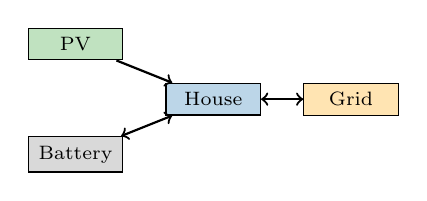
\begin{tikzpicture}[scale=0.7, every node/.style={font=\scriptsize}]
                    \node[draw, fill=pvgreen!30, minimum width=1.2cm] (pv) at (0,2) {PV};
                    \node[draw, fill=storygray!30, minimum width=1.2cm] (bat) at (0,0) {Battery};
                    \node[draw, fill=energyblue!30, minimum width=1.2cm] (house) at (2.5,1) {House};
                    \node[draw, fill=priceorange!30, minimum width=1.2cm] (grid) at (5,1) {Grid};
                    \draw[->, thick] (pv) -- (house);
                    \draw[<->, thick] (bat) -- (house);
                    \draw[<->, thick] (house) -- (grid);
                \end{tikzpicture}
            \end{center}
        \end{column}
    \end{columns}
\end{frame}

% ==============================================================================
% SECTION 6: RESULTS
% ==============================================================================
\section{Optimization Results}

\begin{frame}{Scenario Analysis: PV Low vs. PV High}
    \begin{center}
        \textbf{24-Hour Optimization Results}
    \end{center}

    \vspace{0.5em}
    \begin{table}
        \centering
        \begin{tabular}{lcc}
            \toprule
            \textbf{Metric} & \textbf{PV\_low} & \textbf{PV\_high} \\
            \midrule
            Total Cost (€) & \textcolor{red}{+0.64} & \textcolor{pvgreen}{\textbf{-0.05}} \\
            PV Generation (kWh) & 1.22 & 12.99 \\
            Grid Import (kWh) & 11.16 & 0.00 \\
            Grid Export (kWh) & 0.00 & 0.95 \\
            Self-Consumption (kWh) & 1.22 & 12.04 \\
            Battery Cycles & 1.07 & 0.75 \\
            \bottomrule
        \end{tabular}
    \end{table}

    \vspace{1em}
    \begin{center}
        \colorbox{pvgreen!20}{%
            \textbf{Result: 107\% relative cost reduction from PV\_low to PV\_high!}
        }
    \end{center}
\end{frame}

\begin{frame}{Optimal Dispatch Schedule}
    \begin{columns}[T]
        \begin{column}{0.6\textwidth}
            \begin{center}
                \includegraphics[width=\textwidth]{11_optimization_combined.png}
            \end{center}
        \end{column}
        \begin{column}{0.4\textwidth}
            \textbf{Dispatch Strategy:}
            \begin{enumerate}
                \item \textbf{Morning:} Discharge for peak
                \item \textbf{Midday:} Charge from PV
                \item \textbf{Evening:} Discharge for peak
                \item \textbf{Night:} Minimal import
            \end{enumerate}

            \vspace{0.5em}
            \textbf{Key Insight:}\\
            Battery enables \textbf{arbitrage}.
        \end{column}
    \end{columns}
\end{frame}

\begin{frame}{Scenario Comparison: PV Low vs. PV High}
    \begin{columns}[T]
        \begin{column}{0.5\textwidth}
            \begin{center}
                \textbf{PV Low Scenario}\\
                \includegraphics[width=\textwidth]{11_optimization_PV_low.png}
            \end{center}
        \end{column}
        \begin{column}{0.5\textwidth}
            \begin{center}
                \textbf{PV High Scenario}\\
                \includegraphics[width=\textwidth]{11_optimization_PV_high.png}
            \end{center}
        \end{column}
    \end{columns}

    \vspace{0.3em}
    \begin{center}
        \textbf{Self-Consumption Rate (PV\_high):} $\frac{12.04}{12.99} = \textbf{92.7\%}$ \quad
        \textcolor{pvgreen}{\textbf{Nearly all PV used locally!}}
    \end{center}
\end{frame}

% ==============================================================================
% SECTION 7: CONCLUSION
% ==============================================================================
\section{Conclusion}

\begin{frame}{Summary of Key Findings}
    \begin{columns}[T]
        \begin{column}{0.5\textwidth}
            \textbf{Forecasting:}
            \begin{itemize}
                \item[$\checkmark$] XGBoost outperforms SARIMA by 16\%
                \item[$\checkmark$] Time-of-day is the \#1 predictor
                \item[$\checkmark$] Lag features + exogenous = best accuracy
                \item[$\checkmark$] nRMSE = 0.166 achieved
            \end{itemize}

            \vspace{0.5em}
            \textbf{Data Quality:}
            \begin{itemize}
                \item[$\checkmark$] KNN imputation best for PV gaps
                \item[$\checkmark$] Cyclic encoding captures periodicity
                \item[$\checkmark$] HDD/CDD improve weather signal
            \end{itemize}
        \end{column}
        \begin{column}{0.5\textwidth}
            \textbf{Optimization:}
            \begin{itemize}
                \item[$\checkmark$] LP formulation effectively solves HEMS
                \item[$\checkmark$] 107\% cost reduction (PV\_high scenario)
                \item[$\checkmark$] 92.7\% self-consumption achieved
                \item[$\checkmark$] Battery enables peak shaving \& arbitrage
            \end{itemize}

            \vspace{0.5em}
            \textbf{Business Value:}
            \begin{itemize}
                \item[$\checkmark$] Reduced electricity bills
                \item[$\checkmark$] Increased PV utilization
                \item[$\checkmark$] Lower grid dependency
            \end{itemize}
        \end{column}
    \end{columns}
\end{frame}

\begin{frame}{Limitations \& Future Work}
    \begin{columns}[T]
        \begin{column}{0.5\textwidth}
            \textbf{Current Limitations:}
            \begin{enumerate}
                \item \textcolor{red}{\textbf{Deterministic Model}}
                    \begin{itemize}
                        \item Ignores forecast uncertainty
                        \item No probabilistic bounds
                    \end{itemize}
                \item \textcolor{red}{\textbf{Battery Degradation}}
                    \begin{itemize}
                        \item Cycle aging not modeled
                        \item No capacity fade over time
                    \end{itemize}
                \item \textcolor{red}{\textbf{Perfect Foresight}}
                    \begin{itemize}
                        \item Assumes ideal price forecasts
                        \item No real-time adaptation
                    \end{itemize}
            \end{enumerate}
        \end{column}
        \begin{column}{0.5\textwidth}
            \textbf{Future Improvements:}
            \begin{enumerate}
                \item \textcolor{pvgreen}{\textbf{Probabilistic Forecasting}}
                    \begin{itemize}
                        \item Quantile regression
                        \item Conformal prediction intervals
                    \end{itemize}
                \item \textcolor{pvgreen}{\textbf{Stochastic Optimization}}
                    \begin{itemize}
                        \item Robust MPC framework
                        \item Risk-aware dispatch
                    \end{itemize}
                \item \textcolor{pvgreen}{\textbf{Battery Aging Model}}
                    \begin{itemize}
                        \item Rainflow counting
                        \item Degradation costs
                    \end{itemize}
            \end{enumerate}
        \end{column}
    \end{columns}
\end{frame}

\begin{frame}{Thank You!}
    \begin{center}
        \Huge\textbf{Questions?}

        \vspace{1.5em}
        \large
        \textbf{Samuel Heinrich}\\
        \vspace{0.3em}
        ITS8080 Energy Data Science\\

        \vspace{1em}
        
\begin{tikzpicture}
            \node[draw=energyblue, fill=energyblue!10, rounded corners, minimum width=6cm, minimum height=1.5cm] {\textbf{Interactive Dashboard Demo Available}};
        \end{tikzpicture}

        \vspace{1em}
        \small
        \textit{Code \& Data available in the project repository}
    \end{center}
\end{frame}

% ==============================================================================
% APPENDIX
% ==============================================================================
\appendix

\begin{frame}{Appendix: Project Workflow}
    \begin{center}
        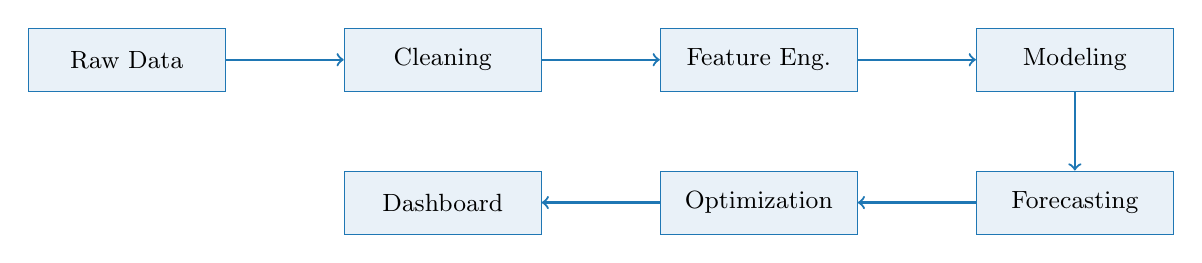
\begin{tikzpicture}[
            node distance=1.5cm,
            box/.style={rectangle, draw=energyblue, fill=energyblue!10,
                        minimum width=2.5cm, minimum height=0.8cm,
                        text centered, font=\small},
            arrow/.style={->, thick, energyblue}
        ]
            \node[box] (data) {Raw Data};
            \node[box, right=of data] (clean) {Cleaning};
            \node[box, right=of clean] (features) {Feature Eng.};
            \node[box, right=of features] (model) {Modeling};
            \node[box, below=1cm of model] (forecast) {Forecasting};
            \node[box, left=of forecast] (optim) {Optimization};
            \node[box, left=of optim] (deploy) {Dashboard};

            \draw[arrow] (data) -- (clean);
            \draw[arrow] (clean) -- (features);
            \draw[arrow] (features) -- (model);
            \draw[arrow] (model) -- (forecast);
            \draw[arrow] (forecast) -- (optim);
            \draw[arrow] (optim) -- (deploy);
        \end{tikzpicture}
    \end{center}

    \vspace{1em}
    \textbf{Notebooks:} 01-11 covering full CRISP-DM lifecycle
\end{frame}

\begin{frame}{Appendix: Mathematical Notation}
    \begin{table}
        \centering
        \small
        \begin{tabular}{cl}
            \toprule
            \textbf{Symbol} & \textbf{Description} \\
            \midrule
            $y_t$ & Actual demand at time $t$ \\
            $\hat{y}_t$ & Predicted demand at time $t$ \\
            $D_t$ & Demand (kWh) \\
            $\text{PV}_t$ & PV generation (kWh) \\
            $G_t^{\text{import}}$ & Grid import (kWh) \\
            $G_t^{\text{export}}$ & Grid export (kWh) \\
            $\text{SoC}_t$ & State of charge (kWh) \\
            $p_t^{\text{buy}}$ & Buy price (€/kWh) \\
            $p_t^{\text{sell}}$ & Sell price (€/kWh) \\
            $\eta$ & Round-trip efficiency \\
            \bottomrule
        \end{tabular}
    \end{table}
\end{frame}

\end{document}
